\documentclass[10pt]{beamer}
\usepackage{ctex}
\usepackage{times}
\usepackage{subfigure}
\usepackage{bm}
\usefonttheme[onlymath]{serif}
\CTEXoptions[today=old]
\usetheme{CambridgeUS}
\usepackage{amsmath}
\setmainfont{Times New Roman}

\begin{document}

\title{Measure Theory}
\author{HaiyangYu \&  WangSong}
\institute[]{Mathematics Institute}
\frame{\titlepage}

\begin{frame}{Introduction}
\begin{columns}
\column{0.65\textwidth}<1->
In mathematical analysis, a measure on a set is a systematic way to assign a number to each suitable subset of that set, intuitively interpreted as its size. In this sense, a measure is a generalization of the concepts of length, area, and volume.(Picture taken from Wikipedia)
\column{0.35\textwidth}<1->
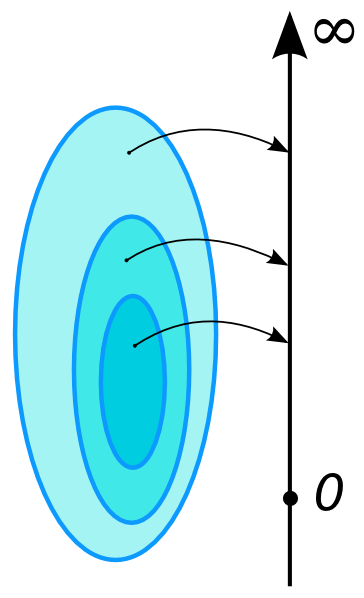
\includegraphics[width=0.9\textwidth,totalheight=0.60\textheight]{1.png}
\end{columns}
\end{frame}

\begin{frame}{Definition}
Let $X$ be a set and ${\varSigma}$ a $\sigma$-algebra over $X$. A function $\mu$ from $\varSigma$ to the extended real number line is called a measure if it satisfies the following properties:
\begin{itemize}
\item{Non-negativity: For all $E$ in $\varSigma$: $\mu(E) \geq0$.}
\item{Null empty set: $\mu( \varnothing ) = 0.$}
\item{Countable additivity (or $\sigma$-additivity): For all countable collections ${\displaystyle \{E_{i}\}_{i=1}^{\infty }}$ of pairwise disjoint sets in $\varSigma$:
    $$\mu\left(\bigcup_{k=1}^{\infty}E_{k}\right)=\sum_{k=1}^{\infty}(E_{k})$$}
\end{itemize}
\end{frame}

\begin{frame}{Examples}
Some important measures are listed here.
\begin{itemize}

\item{The counting measure is defined by $\mu(S) = $ number of elements in $S$.}
\item {The Lebesgue measure on $\mathbf{R}$ is a complete translation-invariant measure on a $\sigma$-algebra containing the intervals in $\mathbf{R}$ such that $\mu([0, 1]) = 1$; and every other measure with these properties extends Lebesgue measure.}
\item{Circular angle measure is invariant under rotation, and hyperbolic angle measure is invariant under squeeze mapping.}
\end{itemize}
\end{frame}


\begin{frame}{Properties}
Let $\mu$ be a measure.
\begin{footnotesize}
\begin{itemize}
\item{Monotonicity: If $E_{1}$ and $E_{2}$ are measurable sets with $E_{1}\subseteq E_{2}$ then $\mu (E_{1})\leq \mu (E_{2})$.}
\item{Subadditivity: For any countable sequence $E_{1}, E_{2}, E_{3}$, ... of (not necessarily disjoint) measurable sets $E_{n}$ in $\varSigma$:
$$\mu\left(\bigcup_{k=1}^{\infty}E_{k}\right)\leq\sum_{k=1}^{\infty}\mu(E_{k})$$}
\item{Continuity from below: If $E_{1}, E_{2}, E_{3},$ ... are measurable sets and $E_{n}$ is a subset of $E_{n+1}$ for all $n$, then the union of the sets $E_{n}$ is measurable, and
    $$\mu\left(\bigcup_{k=1}^{\infty}E_{k}\right)=\lim_{i\rightarrow \infty}\mu(E_{i})$$}
\end{itemize}
\end{footnotesize}
\end{frame}
\begin{frame}
\begin{Huge}
\begin{center}
Thank you!
\end{center}
\end{Huge}
\end{frame}
\end{document}
